\def\mytitle{VECTORE USING PYTHON}
\def\myauthor{SRIKANTH REDDY SURAM}
\def\contact{ssrikanth03@gmail.com}
\def\mymodule{Future Wireless Communication (FWC)}
\documentclass[10pt, a4paper]{article}
\usepackage[a4paper,outer=1.5cm,inner=1.5cm,top=1.75cm,bottom=1.5cm]{geometry}
\twocolumn
\usepackage{graphicx}
\graphicspath{{./images/}}
\usepackage[colorlinks,linkcolor={black},citecolor={blue!80!black},urlcolor={blue!80!black}]{hyperref}
\usepackage[parfill]{parskip}
\usepackage{lmodern}
\usepackage{tikz}
 \usepackage{physics}
\usepackage{karnaugh-map}
\usepackage{setspace}
\doublespacing
%\documentclass{article}
\usepackage{tabularx}
%\usepackage{circuitikz}
\usetikzlibrary{calc}
\usepackage{amsmath}
\usepackage{amssymb}
\renewcommand*\familydefault{\sfdefault}
%\usepackage{watermark}
\usepackage{lipsum}
\usepackage{xcolor}
\usepackage{listings}
\usepackage{float}
\usepackage{titlesec}
\providecommand{\mtx}[1]{\mathbf{#1}}
\titlespacing{\subsection}{1pt}{\parskip}{3pt}
\titlespacing{\subsubsection}{0pt}{\parskip}{-\parskip}
\titlespacing{\paragraph}{0pt}{\parskip}{\parskip}
\newcommand{\figuremacro}[5]{
    
    \begin{figure}
        \centering
        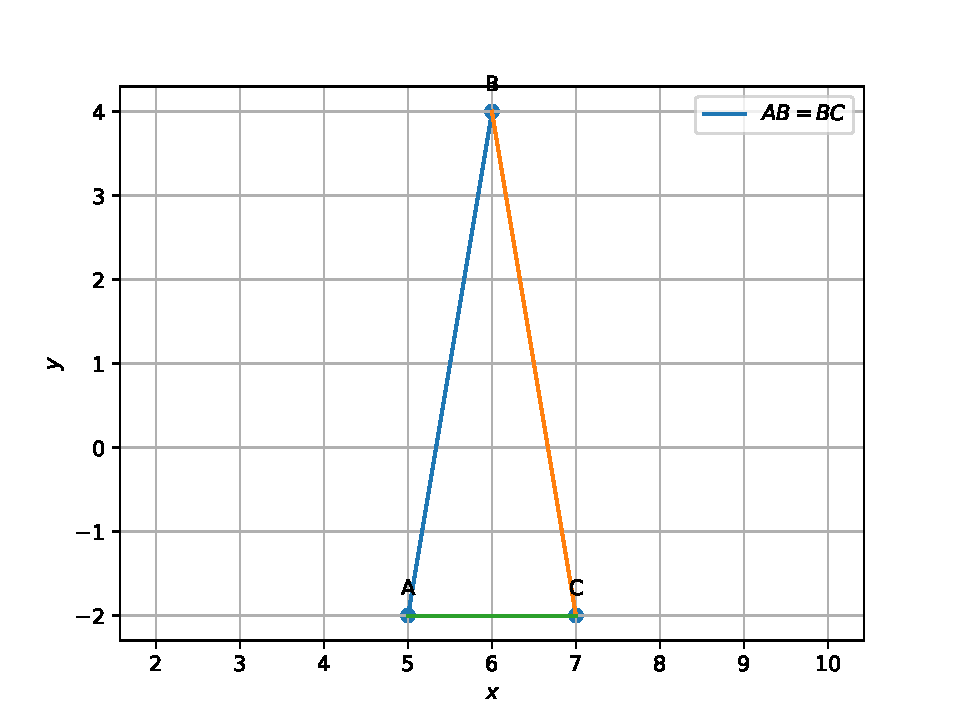
\includegraphics[width=#5\columnwidth]{par.jpg}
        \caption[#3]{\textbf{#3}#4}
        \label{fig:#2}
    \end{figure}
}
\newcommand{\myvec}[1]{\ensuremath{\begin{pmatrix}#1\end{pmatrix}}}
\providecommand{\brak}[1]{\ensuremath{\left(#1\right)}}
\let\vec\mathbf
\lstset{
frame=single, 
breaklines=true,
columns=fullflexible
}
\title{\mytitle}
\author{\myauthor\hspace{1em}\\\contact\\FWC220107\hspace{6.5em}IITH\hspace{0.5em}\mymodule\hspace{6em}ASSIGN-1}
\date{}
\begin{document}
 \maketitle
 \tableofcontents
\section{Construction}                                                                    \begin{center}
  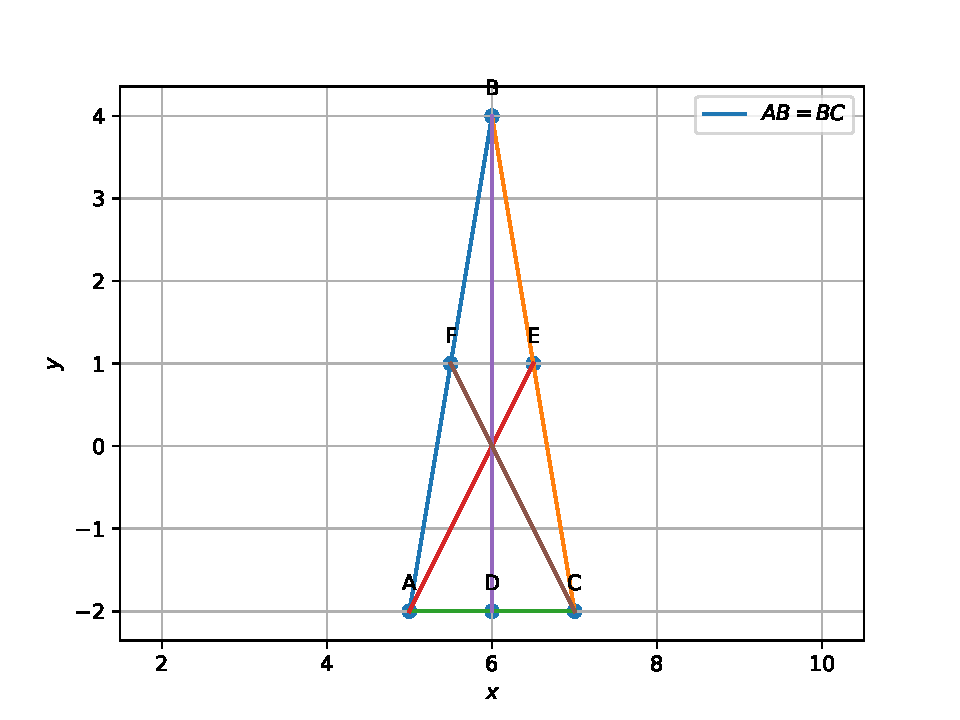
\includegraphics[scale=0.39]{par.pdf}
\\  Figure of construction
   \end{center}
 
   \section{Problem}
  Check whether$(5,-2),(6,4) \text{ and } (7,-2)$ are the vertices of an isosceles triangle.
   
 
Show that the points $\myvec{5, -2}$, $\myvec{6,4}$ and $\myvec{7, -2}$ and vertices of an isosceles  triangle.
	
  \section{solution} Let the given points be $\vec{A}, \vec{B}, \vec{C}$ respectively. 
			 Then, the direction vectors of $AB, BC$ and $CA$ are
\begin{align}
			\vec{A} -\vec{B}&= \myvec{5 \\ -2} -\myvec{6 \\ 4} = \myvec{-1 \\ -6}\\
			\vec{B} -\vec{C}&=  -\myvec{6 \\ 4}-\myvec{7 \\ -2} = \myvec{-1 \\ 6}\\
			\vec{C} -\vec{A}&= \myvec{7 \\ -2} -\myvec{5 \\ -2} = \myvec{2 \\ 0}\\
		From the above,  we find that\\
			\brak{\vec{A} -\vec{B}}^{\top}\brak{\vec{B} -\vec{C}}&=  \myvec{-1 & -6}\myvec{-1 \\ 6}\\
			&=37\\
			\brak{\vec{B} -\vec{C}}^{\top}\brak{\vec{C} -\vec{A}}&=  \myvec{-1 & 6}\myvec{2 \\ 0}\\
			&=-2\\
			\brak{\vec{C} -\vec{A}}^{\top}\brak{\vec{A} -\vec{B}}&=  \myvec{2 & 0}\myvec{-1 \\ -6}\\
			&=-2\\
		From  the above equations, \\
			\brak{\vec{A} -\vec{B}}\perp \brak{\vec{B} -\vec{C}}\\
			\angle BCA = 
			\angle CAB  
\end{align}
		Thus, the triangle is isosceles triangle.

\end{document}

